Last time, we introduced Shannon's Source Coding Theorem:
\begin{thm}
    For an i.i.d (memoryless) source, the optimal rate of reliable data compression (i.e. the data compression limit) is precisely the Shannon entropy $H(X)$ of the source.
\end{thm}

We started by saying that if we have an iid source, we can model it by a collection of $n$ sources $U_1,U_2\ldots, U_n$ which outputs a length-$n$ vector $\underline{u}^{(n)}=(u_1,\ldots, u_n) u_i \in J$. For an iid source, all the sources have the same probability mass function,
\begin{equation*}
    U_i \sim p(u), u\in J,
\end{equation*}
which means that we can equivalently model the source as a single source,
\begin{equation*}
    U\sim p(u), u\in J; p(\underline{u}^{(n)}) =\prod_{i=1}^n P(U_i=u_i)= p(u_1)\ldots p(u_n).
\end{equation*}
The Shannon entropy of the source is given as usal by
\begin{equation}
    H(U)=-\sum_{u\in J} p(u)\log p(u).
\end{equation}

Now let us define a compression map.
\begin{defn}
    A \term{compression map} of \term{rate $R$} is a map $\mathcal C$ with
    \begin{equation}
        \mathcal{C}^n : \underline{u}^{(n)}=(u_1,\ldots, u_n) \mapsto \underline{x}^{m_n}=(x_1,\ldots, x_{m_n}) \in \set{0,1}^{m_n}.
    \end{equation}
    That is, $\mathcal{C}$ maps our output string of length $n$ to a compressed (encoded) string $\underline x$ of length $m_n$. We say that the \term{rate} of encoding is then
    \begin{equation}
        R=\frac{m_n}{n}=\frac{\text{number of bits in codeword}}{\text{number of uses of source}}.
    \end{equation}
    If a compression scheme has rate $R$, then we assign unique codewords to $2^{\ceil{nR}}$ messages.
\end{defn}

Question: when is such a map $\mathcal{C}^n$ a compression map? If our source outputs $n$ values in the alphabet $J$, then we have total possibilities
\begin{equation}
    |J|^n=2^{n\log |J|}.
\end{equation}
These can be stored in $n\log |J|$ bits. Thus $c^n$ is a compression map if $m_n < n\log |J|$, i.e. if we encode the output in fewer bits than it would take to uniquely encode every single string in the naive binary way.

We can of course also define a decompression map:
\begin{defn}
    A decompression map $\mathcal{D}^n$ is a map
    \begin{equation}
        \mathcal{D}^n: \underline{x}^{m_n}\in \set{0,1}^{m_n} \mapsto \underline u^{(n)} = (u_1,\ldots, u_n),
    \end{equation}
    i.e. which takes us back to the original length-$n$ strings of source outputs.
\end{defn}

Now we can ask what the probability of a successful encoding and decoding is-- namely,
\begin{equation}
    \sum_{\underline{u}^{(n)}\in J^n} p(\underline{u}^{(n)}) P\paren{\mathcal{D}^n(\mathcal{C}^n(\underline{u}^{(n)})) \neq \underline{u}^{(n)}}
\end{equation}
is the average probability of error of the compression process. We write this as $P_{av}^{(n)}(C_n)$, where $C_n$ denotes an encoding and decoding scheme.

\begin{defn}
    $C_n$ is a triple defined to be $C_n\equiv (\mathcal{C}^n, \mathcal{D}^n,R)$ which represents a choice of code. We say that a code is \term{reliable} if $P_{av}^{(n)}\to 0$ in the limit as $n\to\infty$. That is, $\forall \epsilon\in (0,1), \exists n$ such that $p_{av}^{(n)} \leq \epsilon$.
\end{defn}

Then there is an optimal rate of data compression,
\begin{equation}
    R_\infty = \inf \set{R : \exists C_n(\mathcal{C}^n, \mathcal{D}^n,R)\text{ s.t. } p_{av}^{(n)}(C_n)\to 0\text{ as }n\to \infty}.
\end{equation}
That is, $R_\infty$ is effectively the minimum rate $R$ of all reliable coding schemes.
What Shannon's source coding theorem tells us is that $R_\infty = H(U).$ The lowest rate (highest density, if you like) we can reliably compress an iid source to is given by the Shannon entropy.

\begin{defn}
    An $\epsilon$-typical sequence is a sequence defined as follows. Fix $\epsilon\in(0,1)$ and take an iid source with $U\sim p(u), u\in J$ which gives us a length-$n$ output $\underline{u}^{(n)}=(u_1,\ldots, u_n).$ Then if
    \begin{equation}\label{epsilontypicalseq}
        2^{-n(H(U)+\epsilon)}\leq p(\underline{u}^{(n)}) \leq 2^{-n(H(U)-\epsilon)},
    \end{equation}
    we say that $\underline{u}^{(n)}$ is an $\epsilon$-typical sequence.
\end{defn}
\begin{defn}
    An \term{$\epsilon$-typical set} is then defined to be the set 
    \begin{equation}
        T_\epsilon^{(n)}=\set{\underline{u}^{(n)}\in J^n\text{ such that }\ref{epsilontypicalseq}\text{ holds}}.
    \end{equation}
\end{defn}

In the asymptotic limit let us observe that
\begin{equation}
    p(\underline{u}^{(n)})\approx 2^{-nH(U)},
\end{equation}
so all $\epsilon$-typical sequences are almost equiprobable since $\epsilon$ can be made arbitrarily small. Does this agree with our intuitive notion of a typical sequence? Yes-- take a sequence $\underline{u}^{(n)}=(u_1,\ldots, u_n), u_i \in J$. %Then the probability of $u$ is 
%\begin{equation*}
%    p(u)\approx \frac{\text{number of times } u\text{ occurs in } \underline{u}^{(n)}}{n}.
%\end{equation*}
Note that for every $u\in J$, the number of times we expect to $u$ to appear in a string $\underline{u}^{(n)}$ is simply $np(u)$.

Our intuition tells us that any typical sequence should therefore fit this expectation.%
    \footnote{To make this more concrete, suppose we have a weighted coin. The weighted coin has outcomes $h$ and $t$ (heads and tails), and it produces $h$ with probability $3/4$ and $t$ with probability $1/4$. If we flip the coin $n$ times, we expect to see about $n\times p(h)=n\times 3/4$ heads and $n\times p(t)= n\times 1/4$ tails since each flip is independent. If $n=4,$ for instance, then a ``typical sequence'' will have three heads and one tails.
    
    Consider a specific example of a length-4 typical sequence, $hhht$ in that order. The probability of getting this specific sequence is $p(h)\times p(h) \times p(h)\times p(t)=27/256$. We could have written this as $(p(h))^{n p(h)}\times (p(t))^{np(t)}$, or equivalently $2^{np(h) \times \log p(h)}\times 2^{np(t) \times \log p(t)}$. Combining terms, we see that this is just $2^{n (p(h) \log p(h) + p(t)\log p(t))}= 2^{-n H(U)}$.
    
    This is not the probability of getting \emph{any} sequence which fits the typical sequence condition! That probability would be something like $\begin{pmatrix}4\\3\end{pmatrix}$ times the probability we got, since we want exactly three heads. However, we will put a bound on this quantity shortly.}
The probability of getting one specific typical sequence is
\begin{align*}
    p(\underline{u}^{(n)}) %&= \prod_{u\in J} \underbrace{p(u)\ldots p(u)}_{n p(u)\text{ times}}\\
    &\simeq \prod_{u\in J} p(u)^{np(u)}\\
    &= \prod_u 2^{np(u) \log p(u)}\\
    &= 2^{n\sum p(u) \log p(u)}\\
    &= 2^{-n H(U)}.
\end{align*}
So this agrees well with our formal definition of a typical sequence. Note that there is a difference between typical and high-probability-- we'll investigate this distinction further on the example sheet.
    
Now, typical sequences have some nice properties.
\begin{thm}[Typical sequence theorem]
    $\forall \delta > 0$ and large $n$,
\begin{itemize}
    \item $H(U)-\epsilon \leq -\frac{1}{n}\log p(\underline{u}^{(n)}) \leq H(u)+\epsilon$%
        \footnote{This follows from taking the log of the definition of an $\epsilon$-typical sequence and dividing by $-n$.}
    \item $P(T_\epsilon^{(n)}) := \sum_{\underline {u}^{(n)}\in T_\epsilon^{(n)}} p(\underline{u}^{(n)}) > 1-\delta$. That is, the probability of getting any typical sequence (as a subset of possible outputs) can be made arbitrarily close to $1$.
    \item $2^{n(H(U)-\epsilon)}(1-\delta) < |T_\epsilon^{(n)}| \leq 2^{n(H(U)+\epsilon)}$, where $|T_\epsilon^{(n)}|$ is the number of typical (length $n$) sequences.%
        \footnote{Since the probability of any individual typical sequence is bounded from below by definition and there are $|T_\epsilon^{(n)}|$ such sequences, the probability of getting \emph{any} typical sequence is bounded by
        \begin{equation*}
            2^{-n(H(U)+\epsilon)} |T_\epsilon^{(n)}| \leq \sum_{\underline{u}^{(n)}\in T_\epsilon^{(n)}} p(\underline{u}^{(n)}) \leq 1.
        \end{equation*}
        This leads us to conclude that $|T_\epsilon^{(n)}| \leq 2^{n(H(U)+\epsilon)}.$
        
        However, $|T_\epsilon^{(n)}|$ is also bounded from below. We know from the previous property and the definition of a typical sequence that 
        \begin{equation*}
            1-\delta < \sum p(\underline{u}^{(n)}) \leq 2^{-n(H(U)-\epsilon)}|T_\epsilon^{(n)}|,
        \end{equation*} so $2^{n(H(U)-\epsilon)}(1-\delta) < |T_\epsilon^{(n)}|.$
        }
\end{itemize}
\end{thm}
%All these properties are collectively known as the \term{typical sequence theorem}.

Since $\epsilon>0,$ we see that in the limit $\epsilon\to 0$,
\begin{equation}
    |T_{\epsilon}^{(n)}| \to 2^{nH(U)}.
\end{equation}
That is, we need $nH(U)$ bits to store all the typical sequences.

Now we can state Shannon's theorem formally.
\begin{thm}[Shannon's Source Coding Theorem]
Suppose we have an iid source $U$ with Shannon entropy $H(U)$.
\begin{enumerate}
    \item (Achievability) Suppose $R>H(U)$. Then $\exists$ a reliable compression-decompression scheme of rate $R.$
    \item (Converse) For $R< H(U)$, any compression-decompression scheme is not reliable.
\end{enumerate}
\end{thm}

\subsection*{Constructive proof of (a)} Let us suppose that $R>H(U)$. We fix $\epsilon \in (0,1)$ such that $R>H(U)+\epsilon$ (for instance, $\epsilon = (R-H(U))/2$). Then we choose $n$ large enough (i.e. the asymptotic limit) such that $T_\epsilon^{(n)}$ satisfies the conditions of the typical sequence theorem. Then we can write
\begin{equation}
    |T_\epsilon^{(n)}| \leq 2^{n(H(U)+\epsilon)}< 2^{nR}.
\end{equation}
Now we divide our set of sequences $J^n$ into the typical set $T_\epsilon^{n}$ and its complement $A_\epsilon^{n}=J^n \setminus T_\epsilon^{n}.$ Let us then order the elements of our typical set, i.e. we assign some labels/indices to all the elements. Since $|T_\epsilon^n| < 2^{nR}$, we need at most $nR$ bits to store all the labels of the typical sequences (i.e. the ones we always want to recover reliably).%
    \footnote{As $nR$ may not be an integer, we'll practically need at most $\ceil{nR}$ bits.}

\begin{figure}
    \centering
    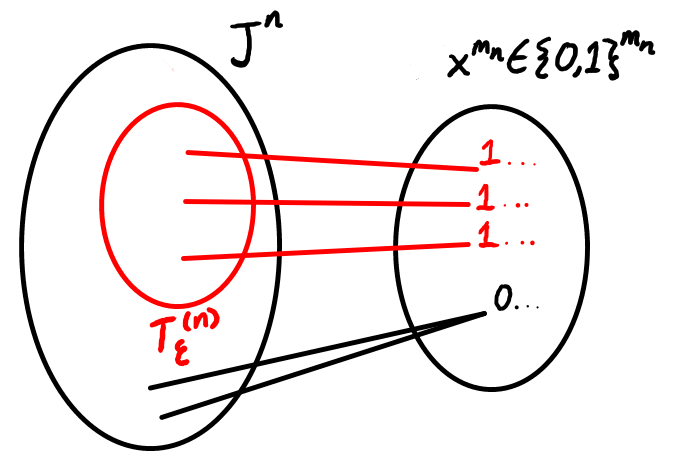
\includegraphics[width=0.75\textwidth]{2019/01/20190121_shannonsourcecoding.png}
    \caption{An illustration of the encoding procedure for the achievability part of the Shannon source coding theorem. Of our source's possible outputs $J^n$, we set up a one-to-one encoding of the typical set $T_\epsilon^{(n)}$, (red ellipse), and send all other elements of $J^n$ to some random value in our set of codewords.}
    \label{fig:shannonsourcecoding}
\end{figure}

With our encoding scheme for the typical set in hand, let us preface our encoding with a $1$, i.e. a \term{flag bit}. So the typical set elements will be encoded as
\begin{equation}
    \underline{u}^{(n)} \in T_\epsilon^n \mapsto 1\underbrace{011\ldots 1}_{\ceil{nR}}.
\end{equation}
Our codewords will be of length $\ceil{nR}+1$, and we can assign the complement $A_\epsilon^n$ to some random codeword beginning with a $0$ instead. This procedure is shown in Fig. \ref{fig:shannonsourcecoding}. So our rate of success when we decode will not be exactly $1$-- we can perfectly decode typical set elements, but there is some loss when we encode elements outside the typical set. However, things are not so bad. Let us take the limit as $n\to \infty$ and look at the failure probability $p_{av}^{(n)}$.
\begin{align*}
    p_{av}^{(n)} &:=\sum p(\underline{u}^{(n)}) P\paren{\mathcal{D}^n(\mathcal{C}^n(\underline{u}^{(n)})) \neq \underline{u}^{(n)}}\\
    &= \sum_{\underline u^{(n)}\in T_\epsilon^n} p(\underline{u}^{(n)}) P(\underline{u}'{}^{(n)}\neq \underline u^{(n)}) 
        + \sum_{\underline{u}^{(n)}\in A_\epsilon^n} p(\underline{u}^{(n)})P(\underline{u}'{}^{(n)}\neq \underline u^{(n)}).
\end{align*}
But the first term is zero since we can always decode typical set elements, and the second part can be made to be arbitrarily small ($<\delta$) by the typical sequence theorem. Therefore we conclude that our scheme is reliable.%
    \footnote{That is, since $P(T_\epsilon^{n}) > 1-\delta$, it follows that $P(A_\epsilon^{n}) < \delta$ in the large-$n$ limit. So the nonzero failure rate is washed out by the fact that
    \begin{equation*}
        \sum_{\underline{u}^{(n)}\in A_\epsilon^n} p(\underline{u}^{(n)})P(\underline{u}'{}^{(n)}\neq \underline u^{(n)}) \leq \sum_{\underline{u}^{(n)}\in A_\epsilon^n} p(\underline{u}^{(n)}) = P(A_\epsilon^{n}) < \delta
    \end{equation*}
    for $\delta$ arbitrarily small.
    } 
\qed

\begin{lem}
    Suppose we have a set $S^n$ which has size $|S^n|=2^{nR}$, with $R< H(U).$ $\forall \delta>0, S_n \subset J^n$ s.t. $|S^n|=2^{nR}$ with $R<H(U)$, we have $P(S^n)< \delta$ for $n$ large enough.
\end{lem}
This implies the converse, and is in the course notes (but is useful to think on by oneself).

\subsection*{Non-lectured aside: the converse} I'll present here an argument for the above lemma. A similar exposition appears in the official course notes.

We have some set $S^n$ with size $|S^n|=2^{nR}$. That is, we can encode and decode at most $2^{nR}$ elements with perfect precision. What elements should we choose?

We know that the probability of our source producing any element in the atypical set $A_\epsilon^{(n)}$ becomes arbitrarily small by the typical sequence theorem, so in order to give our encoding scheme the best chance of success, we should not bother with encoding any elements in $A_\epsilon^{(n)}$.
But note that
\begin{equation*}
    |S^n| = 2^{nR} < 2^{nH(U)} <|T_\epsilon^{(n)}|
\end{equation*}
for some $\epsilon >0$, so we cannot encode the entire typical set. At best, we can encode a subset of $T_\epsilon^{(n)}.$

Let's do that, then. We take $S^n \subset T_\epsilon^{(n)},$ and note that the probability of any individual typical sequence is $2^{-nH(U)}$. Since we have $2^{nR}$ such sequences in $S^n$, the probability of our source producing any sequence in $S^n$ is simply
\begin{equation}
    P(S^n)=\sum_{\underline{u}^{(n)}\in S^n} p(\underline{u}^{(n)})=2^{nR} 2^{-nH(U)}=2^{-n(H(U)-R)}.
\end{equation}
Since $R < H(U)$ by assumption, $H(U)-R > 0 \implies P(S^n)= 2^{-n(H(U)-R)} \to 0$ as $n\to\infty$. Thus $\forall \delta >0$, $\exists N$ such that $P(S^n)< \delta$ for $n\geq N$.

One interpretation of this is as follows-- we tried to encode a subset of the typical set, hoping that any elements in $T_\epsilon^{(n)} \setminus S^n$ wouldn't totally ruin our encoding scheme. However, what we didn't account for was the limit $n\to \infty$. The number of typical sequences grows too fast for our encoding scheme to keep up, so that the probability of our source producing a typical sequence we didn't encode is
\begin{equation}
    P(T_\epsilon^{{n}})-P(S^n) > 1-\delta - 2^{-n(H(U)-R)},
\end{equation}
which can be made arbitrarily close to $1$. The moral of the story is that if we don't encode the entire typical set at a minimum, our scheme is doomed to fail.